%
\chapter{Image Quality Assessment}*
%
Image quality assessment is estimating the frame-by-frame image quality in a video. WRITE ABOUT SECTION LAYOUT AND BRIEFLY WHAT EACH CONTAINS.%This forms the basis for knowing which parts of the videos are suitable for human observation in a final video summary.
%
\section{Literature study}
% kim: findes der ikke andre metoder? (til segmentering) - vi har faktisk kun 2 artikler omkring video kvalitet. resten er om semantisk indhold.
Girgensohn et al.\cite{Girgensohn:2000:SAH:354401.354415} describes a method to measure how shaky a video is frame-by-frame by computing a shift-vector between subsequent frames. They also look into lighting conditions in individual frames by calculating the percentage of pixels within a specific boundary; an indication of reasonable exposure levels in the frame.\\
The \textit{spring loading effect}\cite{Girgensohn:2000:SAH:354401.354415}, also described by Girgensohn et al. is a way to balance clip lengths. It treats the \textit{unsuitability} of the surrounding frames as an additional cost for including them in the clip. The purpose of this is to automatically fit segmented clips to match a desired total clip length.\\
%
A more comprehensive approach described by Wu et al.\cite{10.1109/ICME.2005.1521399} is a multi-level classifier that labels each frame as belonging to one of the groups: \textit{blurred}, \textit{shaky}, \textit{inconsistent} and \textit{stable}. Their solution is based on Support Vector Machines (SVMs) and yield satisfactory results.\\ %Uddybes
LAUGE SKRIVER MERE!
% Lauge: Har fundet to andre artikler om image quality assessment. Skal lige have skimmet dem og sat dem ind her.
%
\section{Method}
%
% kim: skal kunne implementere udfra beskrivelsen af metoden
% NOTE: vi skal have en beskrivelse af hvad vi mener er unsuitable video footage. hvor rystet/mørkt/lyst etc. skal det være for at være unsuitable?
% passer rigtig godt til "intro" afsnittet
%
\subsection{Frame Shift Estimation}
%
We wish to estimate the magnitude of a shift from frame to frame as a measure of how the camera moves. MOAR\\
Girgensohn et al.\cite{Girgensohn:2000:SAH:354401.354415} describes a method that estimates the shift in two subsequent frames, where the direction of a vector is the direction of the shift, and the magnitude of that vector how many pixels was shifted. The advantage of this method is the simplicity in implementation, and low computational costs.\\
We have adopted this method and details are as follows. Each frame is initially shifted 32 frames, as suggested by Girgensohn et al. in four directions (up, down, left, right), halving the number of pixels shifted in each iteration down to 1 pixel.
%The authors suggests a shift of each subsequent frame in four directions of 32 pixels, halving the number of pixels in each iteration to 1 pixel. 
For each shift the Root-Mean-Square (\textit{RMS}) of the difference between the frame and the previous unchanged frame is calculated, and the shift with the lowest \textit{RMS} is the basis for the following iteration. %Shifting a matrix is a simple matter of cutting away parts of the matrix to align the two, and computing the \textit{RMS} is archived in a few inexpensive matrix-computations. Since the frame size of a video determines the amount of movement, which can be detected more or fewer shift-iterations may be better. Girgensohn et al. \cite{Girgensohn:2000:SAH:354401.354415} do not mention the frame size of their videos. We simply stick with the same number of iterations as them, which should be more than enough.\\
%The algorithm below illustrates how the shift vector for two subsequent frames is computed.
\\PASSER DENNE FORKLARING MED NEDENSTÅENDE ALGORITME??? HVIS JA SKROTTER VI ALGORITMEN OG LADER TEKSTEN STÅ.
%
\begin{verbatim}
     f  <- read frame
     f’ <- read frame
     for i in [32, 16, 8, 4, 2, 1]:
          e’ <- infinity
          for d in [left, right, up, down]:
               s <- shift f’ i pixels in direction d
               e <- compute RMS(f-s)
               if e < e’:
                    x,y <- i * (d[x],d[y])
                    e’  <- e
          x’,y’ <- x,y
          f’ <- shift f’ x pixels right
          f’ <- shift f’ y pixels up
     yield x’,y’
\end{verbatim}
%
EVT DROP NEDENSTÅENDE? DET VIRKER LIDT LIGEGYLDIGT\\
A $640\times360$ pixels frame and a frame rate of 24 frames per second (fps) this method can theoretically trace camera movements of up to $24 \times (32+16+8+4+2+1) = 1512$ pixels per second, in any direction, ie. even extremely shaky camera motion should be accurately detected (accuracy is here highly dependant on the blurriness of the frames). Thus, we are able to trace camera movement of more than two full frame widths per second in the horizontal direction and more than three frame heights in the vertical direction.\\\\
%
The \textit{shift vector magnitude ratio}, $S$, is defined as: %as the \textit{shift vector magnitude} normalised into the [0,1] range:
\[
S = (\|v\|)^2 / M^2, 
\]
where $v$ is the \textit{shift vector} (The shift vector magnitude is squared as we wish to increase sensitivity to less desireable values.), and $M$ is the largest possible magnitude of the shift vector. A shift in the same direction in each iteration of the shift vector computation will in our configuration at most shift $32+16+8+4+2+1=63$ pixels.\\
%
\subsection{Frame Contrast Estimation}
%
Girgensohn et al. \cite{Girgensohn:2000:SAH:354401.354415} also describes a method of determining the level of brightness in the image by computing the fraction of pixels above a certain brightness threshold. While this is a sufficient measure for detecting dark images, it does not detect very bright or textureless images, in which features are harder to distinguish. Our method does not have this disadvantage as we compute a measure of contrast in a frame as the standard deviation of the pixel-intensity in the image.
A small standard deviation indicates little contrast/diversity in pixel intensity, ie. a textureless or overly dark/bright image which is less desireable.
A high standard deviation indicates a high contrast/much diversity in pixel intensity, ie. a textured image or an image with a high variation of pixel intensity which is deseriable.\\
% Hence, a very dark image or very bright image would have a low contrast as would images with little or no texture. It will however not detect an image where half of it has a very low contrast, ex. an image of clear sky in the top three-quarters, nor would we necessarily want to discard frames like these.\\\\ % skal vi have et par billeder med deres std. dev. sådan at man kan se med egne øjne, eller er det ikke for simpelt?
% 
% where does this belong (somewhere in algorithms section)
% Another way to compute $v$ is $v = \text{max}(\frac{W_{1}}{T_{1}}, \frac{W_{2}}{T_{2}})$ and $s = v >1$ where $T_{1}, T_{2}$ are the respective lower bounds.
The \textit{contrast} ratio, $C$, is defined as:
\[
C = 1 - (c^2 / N^2),
\]
where $c$ is the standard deviation of the pixel intensity in a frame ($c$ is squared as we wish to increase sensitivity to less desireable values), and $N$ is the largest possible value of $c$. The pixel intensity is in the range $[0,255]$ (grayscale image), hence $N$ is at most $127.5$ (an image-matrix exclusively containing values of 0 and 255 in an equal amount). $c \to N$ indicates a high quality image, but as we wish that $C$ is compareable to $S$ where a value of $S$ close to 0 is desireable $c/N$ is substracted from $1$.\\
%
\subsection{Triangular Smoothing}
%
%There are several approaches to computing the suitability for a given frame: A binary approach in which a frame is simply deemed suitable or unsuitable for watching, and an approach where a frame is rated on a scale. These are discussed in detail in section REFERENCE TO SECTION "The Algorithms".
%
%The values of these variables are quantified as how bad they are compared to how bad they can be.\\
%
%
%
Finally $S$ and $C$ are smoothed using \textit{trianglur smoothing} with a degree of $12$ in order to remove outliers. Triangular smoothing is a weighted smoothing function where the degree of smoothing determines the distribution of weights. As the name suggests the weights are distributed in a triangular fashion where the highest weight is the middle one and the remainder of the weights diminish in a linear fashion as a function of distance from the middle. Triangular smoothing can then be described by:
%
\[
s_{j} = 
\begin{cases}
\frac{\sum_{i=0}^{2d} w_{i}x_{j+i-d}}{T} & j=\{1,\dots,n-1\}\\
x_{j} & j=\{0,n\}
\end{cases}
\]
%
where $d$ is the degree of smoothing, $w$ is the weight, $x$ is the value in the original data, $T = \sum_{i=0}^{2d}(w_{i})$ ie. the triangle sum, and $s$ is the smoothed value. HOW TO EXPLAIN BORDERCASE WHERE TRIANGLE IS OUTSIDE DATA-RANGE? %If the subscript of $x$ is negative the triangle is decreased accordingly in size. VI LADER DEN LIGE LIGGE\\
%
\subsection{Frame State Classification}
%
The methods described in section \ref{sec} are all functions of the shift vector magnitude ratio and contrast ratio, and one or more tresholds. Each method computes a suitability measure, $v$, of the frame, and the frame state is then classified as:
\[
s = 
\begin{cases}
1 & \text{ if } v \leq 1\\
0 & \text{ otherwise }
\end{cases},
\]
unless otherwise noted. Where $s=1$ is a positive classification, and $s=0$ is a negative classification.
% where $0$ is a less desireable frame state, and a frame state of $1$ is desireable.
\subsection{Algorithms - RENAME?}
%
\subsubsection{Contrast Only RENAME?}
%
%This method ignores shift magnitude ratio, $S$, 
The frame state, $v$, is defined as $v=\frac{C}{\tau}$, %, and the frame state, $s$, is classified as follows:
% \[
% s = 
% \begin{cases}
% 1 & \text{ if } v \leq 1\\
% 0 & \text{ otherwise }
% \end{cases},
% \]
%
where $\tau$ is some treshold.
%
\subsubsection{Shift Magnitude Only RENAME?}
%
The frame state, $v$, is defined as $v=\frac{S}{\tau}$, %, and the frame state, $s$, is classified as follows:
%This method ignores the contrast ratio, $C$, and marks the frame state, $s$, as follows
% \[
% s = 
% \begin{cases}
% 1 & \text{ if } v \leq 1\\
% 0 & \text{ otherwise }
% \end{cases},
% \]
%
where $\tau$ is some treshold.
%This algorithm only considers how much a frame was shifted in order to attempt to match it to the frame before it. That is, it only looks at how much the images are moving or shaking. Just like with the CO algorithm we simply measure if the \textit{shift vector magnitude} is beyond the configured limit, and mark the frame good or bad accordingly.
%
\subsubsection{Independent Contrast and Shift Magnitude RENAME?}
%
%This algorithm takes both parameters into consideration and looks at if any of the two exceeds a given threshold. 
This methods ignores the cumulative effect of the contrast and shift vector magnitude ratio, and is simmilar to the approach taken by Girgensohn et al. \cite{Girgensohn:2000:SAH:354401.354415}. The frame state, $v$, is defined as $v=\text{max}(\frac{C}{\tau_1}, \frac{S}{\tau_2})$,%, and the frame state, $s$, is classified as follows:
%This mean that we ignore the cumulative effect of the two as a determinant for whether the video segment is unsuitable. This is simmilar to the approach taken by Girgensohn et al. \cite{Girgensohn:2000:SAH:354401.354415}. The frame state is marked as follows:%classifier, \text{S(c,s)}, is defined as:
% \[
% % S(c,s)=MAX(c \cdot (1-c_{lim}), s \cdot (1-s_{lim}))
% s=
% \begin{cases}
% 1 & \text{ if } v \leq 1\\
% 0 & \text{ otherwise }
% \end{cases},
% \]
where $C$ is the contrast ratio, $S$ is the shift vector magnitude ratio, $\tau_1$ and $\tau_2$ are some tresholds.
%where \text{c} and \textit{s} are the \textit{contrast-} and \textit{shift vector magnitude}-ratios respectively and $c_{lim}$ and $s_{lim}$ are the limits defined by our configuration. 
The function effectively normalises the effect of the tresholds LAUGE UDDYBER.% so that the two values can be compared by the \textit{MAX} statement. 
%If $S(c,s) > 1$, one of the two parameters is beyond its limit and the frame is marked as bad.\\\\
%
\subsubsection{Cummulative Contrast and Shift Magnitude RENAME?}
% ANDERS
This method investigates the cumulative effect of both ratios, but we still wish that either one of them can mark a state on its own, as explained below. The frame state is marked as follows:\\
% With this method we ensure that either factor will be able to deem a frame unsuitable, and if both weights are close to their respective treshold the cumulative contribution will still deem the frame unsuitable.
\[
s = v \ge \tau,
\]
where 
%If $S$ is the shift vector magnitude ratio, $C$ is the contrast ratio, $s$ is either 1 (suitable) or 0 (unsuitable), and $v$ is a measure of suitability, then 
%$v$ is defined as: 
$v = \alpha S + \beta C$, and $\alpha,\beta$ are weight-factors, and %and $s$ is then determined by $s \equiv v \ge \tau$, where 
$\tau$ is some treshold. If we wish that $s \equiv S \ge \tau_{1} \vee C \ge \tau_{2}$ it follows that
%
\[
 \alpha S + \beta C \ge \tau \equiv  S \ge \tau_{1},
\]
%
ie. if $S$ is greater than the treshold $\tau_{1}$ then $\alpha S + \beta C$ must also be greater than the treshold $\tau$.% , the values of $\alpha$ and $\beta$ are determined as follows:
%the point being that the contribution from $S$ alone can determine the outcome of $s$, 
 We set $C = 0$ and $S$ assumes the lowest possible value, $S = \tau_{1}$, and we can determine the value of $\alpha$ as:
%
\[
\alpha \tau_{1} \ge \tau \Leftrightarrow \alpha \ge \frac{\tau}{\tau_{1}}
\]
%
It follows that the value of $\beta$ can be determined as $\beta \ge \frac{\tau}{\tau_{2}}$.
\\NOGEN DER FATTER DETTE? ER VORES VINDERALGORITE....
%
%Another approach is $v = (a^x + b^x)^{\frac{1}{x}}$ for a given value of $x > 1$, and then testing $v$ against a given treshold, $\tau$. It is somewhat similar to the previously mentioned approach where we multiply by some factor, and then add the values, the difference being that large values will weigh much more than small ones.
%
% \paragraph{Simplified contrast and shift magnitude ($\text{CCSM}^{3}$)}
% %
% The last algorithm is a very simplified version of \textit{CCSM}. It attempts to classify the frames by simply taking the mean of \textit{contrast} and \textit{shift vector magnitude} and checking to see if it above a given threshold. The frame state classifier, \text{S(c,s)}, is defined as:
% \[
% S(c,s)=\sqrt[3]{\frac{c^{3}+s^{3}}{2}}
% \]
% The parameter values are cubed (and the result normalised to the [0,1] range) in order further increase their sensitivity toward bad values. Informal experimentation shows that the power of sensitivity does not effect the outcome result in any significant way, so it has been left out as a parameter.
%
\section{Dataset}
%
% Most of the videos in this dataset was found on YouTube and collected as described in section \ref{sec:dataset}.\\
This section mentions details that about our dataset that is only relevant for image quality assesment. We can categorize the videos from YouTube as unedited video and pre-edited video where the non-edited video is the most desireable as this is presumeably raw footage.
%What we generally want is raw video, but since this is by far the lesser portion of the two we use the pre-edited video as a sort of benchmark on the pretense that a large majority of the footage is both of high quality and also contextually interesting.\\
%
\paragraph{Unedited YouTube Videos}
%
The dataset contains 25 raw videos. The length of the clips range from 10 seconds to 10 minutes, totaling somewhere around one hour of footage. \textbf{Lauge: Disse tal skal opdateres så vi er sikker på at de stemmer overens med det vi rent faktisk har}
% Lauge: Disse tal skal opdateres så vi er sikker på at de stemmer overens med det vi rent faktisk har
All videos appear to have been recorded using hand-held devices so the quality of the footage varies a lot. In order to be able to train and test on this part of the data set, we generate a \textit{gold standard} manually for each video, by watching the video and marking sections of high and low quality. %This is done by watching the video and recording every time the footage switches state from \textit{bad} to \textit{good} or vice versa.
%
\paragraph{Pre-edited Youtube videos}
%
%The dataset furthermore contains a alot pre-edited videos. This is because far the m
Most videos available on Youtube have already been edited in some way. 
%Many of these videos consist of several different video-clips, which themselves was once raw footage. 
In order to use these clips we cut these pre-edited videos into multiple videos at their scene boundaries. The editing is done manually without too much concern of loosing a few hundred milliseconds of footage the scene boundaries in order to speed up editing. Some of these scenes are undesireable, such as scenes with much on-screen text, credits, montages, ie. scenes that would not be considered raw footage. Also very short scenes are discarded. Because the resulting set of videos have already been screened and deemed watchable by a human (the producer of the video), we assume that all of this footage is a \textit{gold standard} in regards to later testing.
%This is done manually in much the same way as the when generating the \textit{gold standard} for the raw Youtube videos; by watching the videos and marking the points of change of scene. 
%Since a lot of these edited videos contain (for our purpose) unsuitable footage, like photos or on-screen text, only the parts that actually depict the event is kept. Because the resulting set of video-clips have in fact already been screened and deemed watchable by a human (namely the producer of the edited video), we assume that all of this footage is of a decent quality. During review we discard some of the the segmented video-clips, namely:
% ALLEREDE NÆVNT
% \begin{itemize}
% \item very short segments - usually a 1 second segment would be discarded
% \item contextually invalid - ex. a montage of still-images or ending credits
% \item lack of visual quality - in some extreme cases an entire segment can be extremely dark/bright or shaky. This is obviously not acceptable since we assume all these segments to be of a decent quality in our later tests.
% \end{itemize}
%
%Keep in mind that some of these segments are discarded as they are out of context of the entirety of the video-clip, where they would (presumably) make sense to include, but not as standalone segments.\\
We also accept some \textit{noise} in each end of the segment to complement ex. overly long crossfades. LAUGE %In the end we end up with a large selection of short segments of video-footage that we expect to be of good quality.
%
\paragraph{Own recordings}
%
The dataset also contains five videos, which we have recorded ourselves. These videos depict various specific scenarios involving low contrast and darkness, shakiness, fast camera movement and completely still footage. These videos serve as a starting point for parameter tuning. They are however not used in later phases.
%
\section{Findings}
%
Due to a limited size dataset we perform a k-fold cross validation, described in section \ref{sec:kfoldxval}. The metric of success is whether a method correctly estimates the quality of a frame, in respect to the \text{gold standard}, and the parameters used in the specific configuration of that method. We investigate both the performance of various methods, and also their robustness as a measure of how sensitive they are to parameter change.\\
For each algorithm we determine the optimal configuration of parameter(s) using k-fold cross validation, where the optimal configuration is the one that has the lowest distance score, described in section \ref{sec:ph1tweaking}. We also record some of the side-effects of each configuration such as the average length of a...\\
Obviously, we want the resulting distance-score to be as small as possible as this signifies a good performance, but we also try to capture some of the side-effects of the specific configuration. One of the things we are interrested in knowing is how many frames long the average good video-clip is. This in itself does not tell us much, since even a very good classifier could end up with very short video-clips if the footage it was classifying is very bad. However, if several algorithms perform equally well this could work as a tie-breaker, as we in general prefer long good-quality clips since they give us more room for manoeuvre later on when we have to actually segment the footage. The variance of this length along with the median lenght is also calculated.
%Our tests attempts to estimate several different algorithms overall ability to correctly estimate the qualities of the frames in a video and classify them as either good or bad. Further more we want to estimate what parameter(s) yield the best performance for each algorithm.
%The dataset is trained using 5-fold cross validation (described in detail in the following). 
%
\subsection{K-fold Cross Validation}\label{sec:kfoldxval}
%
 In k-fold cross validation the dataset is randomly partitioned into $k$ subsets of which one is retained for testing the method and the remaining $k-1$ subsets are used for training. The cross validation is repeated $k$ times where each of the subsets are used only once for testing. The resulting score and parameter(s) from each fold is averaged. % VI SKAL LIIIIIGE KIGGE PÅ OM ALT DETTE ER KORREKT. MEN K-FOLD X-VAL. ER DOG BESKREVET I "DETALJER".
%The cross-validation process is then repeated k times (the folds), with each of the k subsamples used exactly once as the validation data. The k results from the folds then can be averaged (or otherwise combined) to produce a single estimation. The advantage of this method over repeated random sub-sampling is that all observations are used for both training and validation, and each observation is used for validation exactly once. 10-fold cross-validation is commonly used[5], but in general k remains an unfixed parameter
%Since our dataset is limited in size we perform 5-fold cross validation on it in order to increase the amount of videos in the training set. 
%
%The dataset is split into five buckets by sorting the video-clips by length and inserting them, one at a time, in a circular manner. The result is five sub-sets each containing more or less the same amount of frames between all the videos in each set. We then tweak each algorithm's parameter(s) on each of the training sets created by combining four out of the five sub-set and subsequently test the configuration on the remaining test set (the remaining fifth sub-set) and average the results into final scores. 
%We also attempt to estimate how \textit{robust} each algorithm is against changes to its parameter(s). That is, we want to quantify how good the algorithm is overall. This analysis is based on the entire dataset and happens after the 5-fold cross validation.
%
\subsection{Parameter tuning}\label{sec:ph1tweaking}
%
Parameter tuning is often a matter of maximising positive precision and recall. Positive precision is the certainty at which we can say that a positive classification is correct, whereas positive recall is the ratio of true positives we find compared to how many actually exists. Relative Operating Characteristics (ROC) diagrams, as described by Fawcett\cite{Fawcett06a}, is a useful tool for quantifying the overall stability of an algorithm. The ROC diagrams plot different parameter configurations as the relation between the resulting \textit{true positive rates} (the benefit) and \textit{false positive rates} (the cost). Plotting this relation yields a curve, whos underlying area can be used as an estimate of the algorithms stability, where a large area indicates a stable algorithm, and a small area indicates an unstable algorithm.\\
% Lauge: Vi skal sgu nok lige smide en lille figur ind her...
However, due to the disproportion in frame states in our dataset (there is a relative high amount of high quality footage), this approach is not suitable in our case. We want to maximise the positive precision and negative recall. BEDRE FORKLARING HER: Effectively, this means that we reward methods, that are not only good at avoiding unsuitable frames, but also delivered mostly true-positive good frames. We are willing to do this at the cost of dismissing some of the suitable frames. However, in order to limit this \textit{waste} we still consider low positive recall and low negative precision a cost, which should be limited. Inspired by the structure of ROC diagrams we established our own meassuring tool. However, in our case the cost, \textit{C}, and benefit, \text{B}, are defined as:
% \[
% C = 1 - 2 \cdot \frac{positive_{recall} \cdot negative_{precision}}{positive_{recall} + negative_{precision}}
% \]
\[
C = 1 - 2\frac{P_{r}N_{p}}{P_{r} + N_{p}},
\]
and
% \[
% B = 2 \cdot \frac{negative_{recall} \cdot positive_{precision}}{negative_{recall} + positive_{precision}}
% \]
\[
B = 2\frac{N_{r} P_{p}}{N_{r} + P_{p}}
\]
where $P_r$ is positive recall, $N_p$ is negative precision, $P_r$ is positive recall, and $N_p$ is negative precision.\\
%
In both cases we combine the two influencing parameters by calculating their harmonic mean. We want \textit{C} to be as small as possible and \textit{B} to be as large as possible. In the final step we visualise this, by plotting the result of different parameter setting in a ROC-like diagram. The costs and benefits are plotted along the two axis, and as with a normal ROC diagram we want the points to lie as close to the top left corner as possible, as this signifies a large benefit with a small cost. From this diagram we are able to estimate the specific algorithms overall performance, across many different choices of parameter values, by calculating the area under the curve the plots form. However, we are also able to identify the single best parameter choice. We do this by calculate the distance from each point to the [0,1] coordinate (the optimal configuration) and use it as a final score. The smaler the score, the more optimal the configuration is.\\\\
%
NOTE: There actually is a problem with calculating the score this way. We have come up with another method which should be mathematically sound, but too late in the process to change anything.\\\\
% Noter fra Kim: What? Hvorfor ikke areal? Forklar!
% Lauge: Der er faktisk nogle ting vi lige skal have overvejet med det her. (Se notesbog!)
%
\begin{figure}
     \centering
     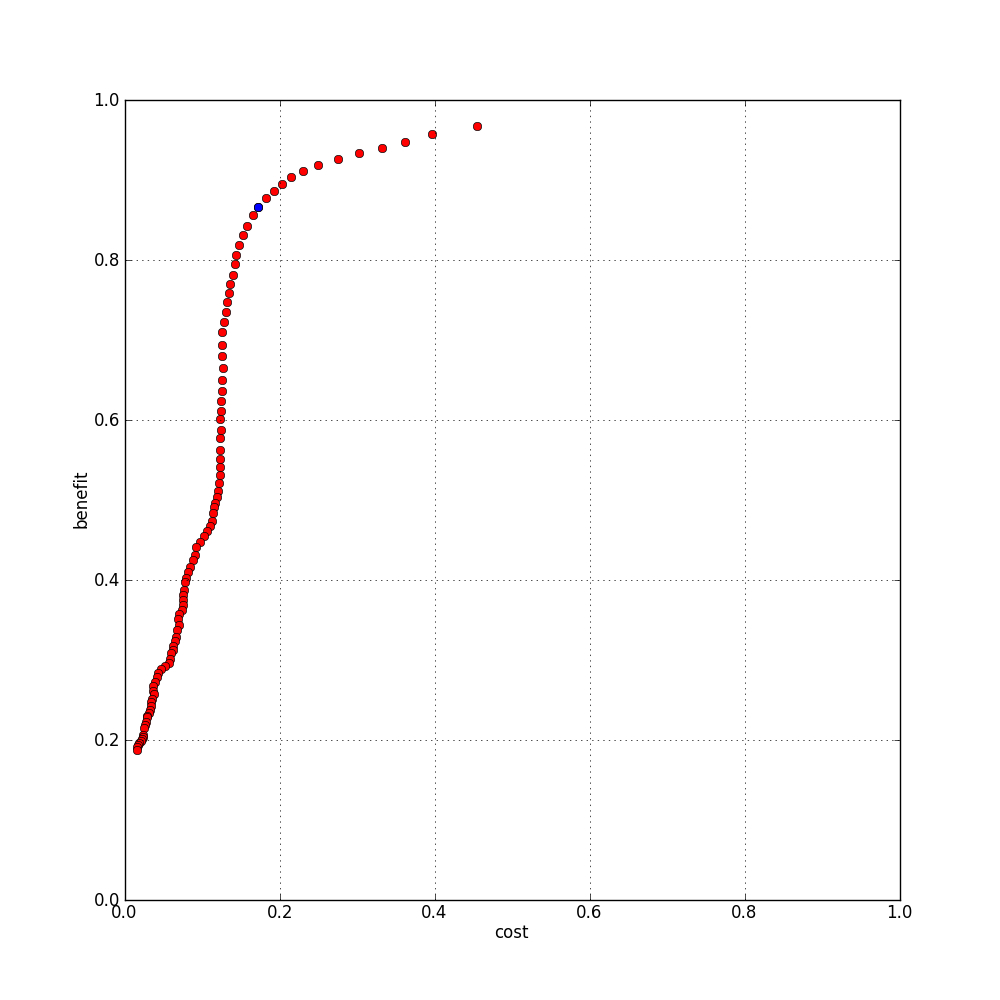
\includegraphics[width=0.75\textwidth]{img/2dcostbenefitexample2.jpg}
     \caption{An example of a 2D cost/benefit diagram, the blue configuration is the one with the lowest distance score}
\end{figure}
%
% \subsubsection{Testing RENAME}
% ANDERS
%
\subsection{Robustness}\label{sec:robustness}
%
On top of the ordinary parameter tuning and testing we also attempt to measure the overall robustness of each of the algorithms with respect to the change of parameter. This is done by calculating the area under the curve (AUC) of the cost/benefit diagrams generated by each algorithm. For this we use the entire dataset, which is to say that it happens after the 5-fold cross validation. Any algorithm, whos benefit-value is generally larger than its corresponding cost-value, across all choices of parameter(s) will have an AUC larger than 0.5. The larger the AUC is the more robust the algorithm is toward changes to its parameter(s). Since the points produced by most of the algorithms are not evenly spread over the entire diagram, we insert points at the (0,0) and (1,1) coordinate in order to cover the entire span of the diagram along the x-axis. It can be argued whether this is the most correct way to handle this, but it does produce comparable AUCs across all algorithms. Unlike the tweaking and testing described above this does not tell us anything useful about the best parameter to choose since we have no way of knowing how this would generalise. But it does tell us something about the nature of the algorithm itself. In general we would prefer our algorithm of choice to be as robust as possible as it signifies a sensible selection of parameters. 
%
\subsection{Multi-parameter algorithms}\label{sec:ph1multiparameter}
%
All our algorithms, except one, only have one parameter. This makes them easy to tweak and test and also very straightforward to generate cost/benefit diagrams for. The \textit{ICSM} algorithm, however, has two parameters and this causes some problems. First and foremost the additional parameter makes tweaking much more computational expensive. With the other algorithms we tweak the one parameter by one percentage point in each iteration, which limits the number of configuration to a hundred. To do so with the \textit{ICSM} algorithm would require 10.000 tweak iterations, which is much too expensive even when the results of intermediate calculations are cached on disk. In order to bring this number down we start we start out by attempting to learn something about the base characteristics of the algorithm by probing it using some uniformly selected configurations. In the case of the \textit{ICSM} algorithm we see that the \textit{contrast} parameter has a huge influence on how well the algorithm is defined in the cost/benefit spectrum. For very low values of \textit{contrast} almost all results are undefined because all frames are marked as good, which makes it impossible to calculate precision and recall correctly. On the other end of the spectrum, when \textit{contrast} is large, the effect of changing it is very small, signifying that it converges toward some optimal value. Based on this information we choose to decrease the precision with which we tweak \textit{contrast} to ten percentage points per iteration. This brings the total number of tweak iterations down to 1000. This still takes a long time, but it is manageable.\\
\\
The second problem is encountered when generating the cost/benefit diagrams and calculating the AUC. The effect of changing more than one variable is not illustrated very well in a two-dimensional cost/benefit diagram. The points, which really belong in a higher dimensional space, are flattened into the plane resulting in several curves without any clear connection to each other. This also causes problems when calculating the AUC for the algorithm, since curves generated by bad performing configurations can be hidden below curves generated by good performing ones, which in the end results in a over-optimistic robustness score.
%
% \begin{figure}
%      \centering
%      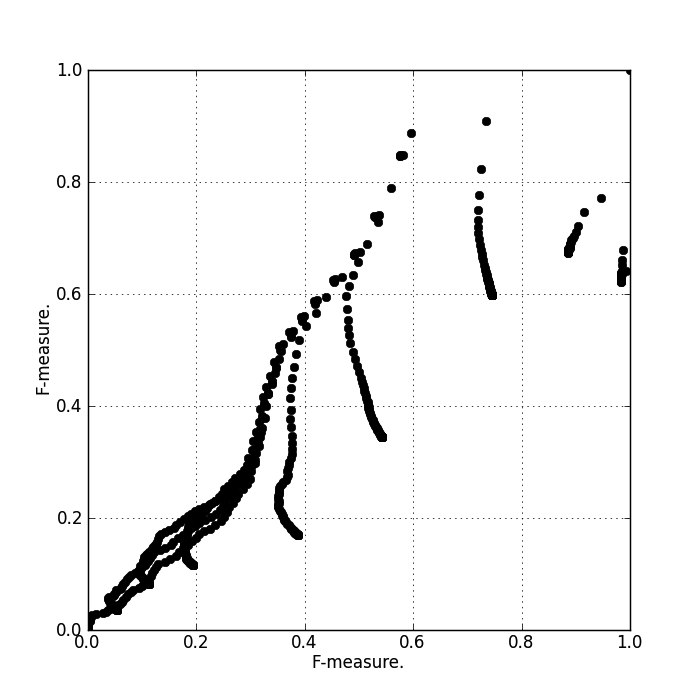
\includegraphics[width=0.75\textwidth]{img/2dcostbenefitexample.jpg}
%      \caption{An example of a 2D cost/benefit diagram for an algorithm with two variables}
% \end{figure}
%
%
% Noter fra Kim: Y-axis = benefit? X-axis=cost? Ser mærkeligt ud, drop!
%
In order to overcome this problem we simulate having only one parameter by locking the second one (contrast) to a specific value and then performing our analysis as usual. We repeat this over and over again, locking the contrast parameter to a new value in each iteration until we have covered all configuration combinations. For the robustness analysis we then add an aditional axis, representing the locked parameter, to our cost/benefit diagram and draw our points in three dimensions. The plane created illustrates the robustness of the algorithm much better. Since the choice of contrast values across all iterations are uniformly distributed, we can easily determine the AUC for the algorithm by simply calculating the individual AUCs for each selection of contrast value and compute an average.
%
\begin{figure}
     \centering
     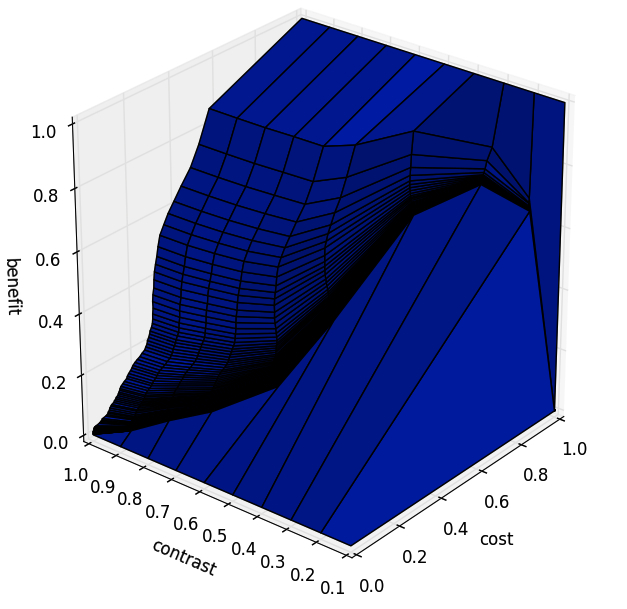
\includegraphics[width=0.75\textwidth]{img/3dcostbenefitexample.jpg}
     \caption{An example of a 3D cost/benefit diagram}
\end{figure}
%
% \subsubsection{Test cases}\label{sec:testcases}
%
\subsection{Frame by frame classification (FFC)}\label{sec:fbfclass}
%
The first test case only looks at each frame independently. For each frame we determine the level of contrast and the shift vector magnitude and use this information alone to perform a binary classification of the frame as \textit{good} or \textit{bad} using the algorithms described above. The results are compared with our \textit{gold standard} for the videos and the amount of true and false positives and negatives are used to calculate precision and recall for both classes.
%
\subsection{Temporal classification (TC)}\label{sec:tempclass}
%
In the second test case we change the way we punish misclassifications. We instead consider the videos as switching back and forth between two states, \textit{good} and \textit{bad}. Misclassifications, which happen close to these change-of-state's are punished less than those that happens elsewhere. The rationale behind this is that it is very difficult to objectively determine the exact point (frame) where a human observer will consider the quality of a video as changing from one state to the other. Likewise, we expect a human observer to ignore very short sub-parts of good or bad quality footage, if it is surrounded by a significant amount of footage of the opposite type. Overall, we want to be more tolerant of misclassifications, where it makes sense. For this we need a more advanced \textit{penalty function} than the simple binary check from the FFC test case.\\
%
We start by identifying all the positions in the sequence of frames where the state changes from good to bad or vice versa. Let $S$ be the set of all these positions. Also let $x$ any position in the video and let $c$ be some level of tolerance for mistakes. A \emph{penalty function} for determining the ratio of punishment for a misclassification at position $x$ is then defined as:
%
\begin{displaymath}
P(x) =1 - MAX_{s\in S}(e^{-\frac{(x-s)^{2}}{2c^{2}}})
\end{displaymath}
%
This function places a series of inverted gaussian bell curves at the point of every change of state. Figure \ref{fig:penaltycurve} shows an example of this. The value $c$ defines the width of the curve and thus determines how tolerant we are.
%
% Noter fra Kim: Valgt hvordan?
%
\begin{figure}
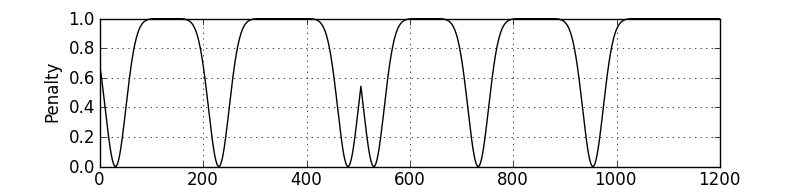
\includegraphics[width=1\textwidth]{img/penaltyfunction.jpg}
\caption{An illustration of a curve generated by the penalty function P}
\label{fig:penaltycurve}
\end{figure}
%
\emph{P(x)} always returns a value between 0 and 1, that tells us how severe a misclassification at position $x$ is. All correct classifications are treated just like in the FFC test case. However, if a misclassification occurs, we look at the \textit{penalty function} to see how the classification should be scored. There is one problem with this appraoch. It makes maintaining accurate true- and false- negative and positive values slightly less trivial. If a misclassification occurs at frame \textit{x} and \emph{P(x)} is very close to 0, how true (or false) is the classification)? The way we handle this is simply by adding \textit{P(x)} to the \textit{false} ratio for this type (positive or negative) and \textit{1 - P(X)} to the opposite type. That is, we quantify the classification as being both true and false to a varying degree determined by the \textit{penalty function}.
%
\subsection{Smoothing of the algorithm suggestions}\label{sec:classsmooth}
%
Finally, for both algorithms, we also investigate the effect of smoothing the classification results. This is done to remove outliers in the final results and should not be confused with the smoothing of the \textit{contrast} and \textit{shift vector magnitudes} in the algorithms themselves.
%
\subsection{Results}
% ANDERS
Table \ref{tab:algoconfigs} shows the different algorithm configurations. \textit{Label} is the specific algorithm configurations name. \textit{Algorithm} is the specific algorithm. \textit{Smoothness Degree} is a measure of how much the algorithm result is smoothed as described in \ref{sec:classsmooth}. \textit{Comparison Method} indicates if the algorithm result is compared using Frame-by-Frame Classification as described in section \ref{sec:fbfclass}, or using a Temporal Classification, as described in \ref{sec:tempclass}, using the stated \textit{Tolerance}. \textit{Parameter} is the parameter configuration for a given algorithm.\\
A final configuration of an algorithm is hence a smoothness degree for smoothing the resulting frame states and a set of parameters, and which method was used to tune this configuration in respect to the gold standard.\\
Algorithm configuration and configuration is used interchangeably in the following.
%The parameter is the average over the 5-fold cross validation. Smoothness degree describes how much the result is smoothed using triangular smoothing. The comparison method is either frame-by-frame (FFC) or temporal (TC), both described in section \ref{sec:testcases}.\\
%
\begin{table}[h]
  \begin{tabular}{| l | l | p{2cm} | p{2cm} | c | c | }\hline
    Label & Algorithm & Smoothness degree & Comparison method & Tolerance & Parameter(s)\\\hline
    ICSM1 & ICSM & 0 & FFC & N/A & (0.052, 0.720) \\\hline
    ICSM2 & ICSM & 12 & FFC & N/A & (0.054, 0.720) \\\hline
    ICSM3 & ICSM & 0 & TC & 24 & (0.060,0.720) \\\hline
    ICSM4 & ICSM & 0 & TC & 48 & (0.064,0.720) \\\hline
    ICSM5 & ICSM & 12 & TC & 24 & (0.058,0.720) \\\hline
    ICSM6 & ICSM & 12 & TC & 48 & (0.064, 0.720) \\\hline
    ICSM7 & ICSM & 0 & TC & 12 & (0.056, 0.720) \\\hline\hline
%
    CCSM1 & CCSM & 0 & FFC & N/A & 0.092 \\\hline
    CCSM2 & CCSM & 12 & FFC & N/A & 0.088 \\\hline
    CCSM3 & CCSM & 0 & TC & 24 & 0.100 \\\hline
    CCSM4 & CCSM & 0 & TC & 48 & 0.108 \\\hline
    CCSM5 & CCSM & 12 & TC & 24 & 0.094 \\\hline
    CCSM6 & CCSM & 12 & TC & 48 & 0.110 \\\hline
    CCSM7 & CCSM & 0 & TC & 12 & 0.098 \\\hline\hline
%
    CO1 & CO & 0 & FFC & N/A & 0.462 \\\hline
    CO2 & CO & 12 & FFC & N/A & 0.460 \\\hline
    CO3 & CO & 0 & TC & 24 & 0.466 \\\hline
    CO4 & CO & 0 & TC & 48 & 0.474 \\\hline
    CO5 & CO & 12 & TC & 24 & 0.468 \\\hline
    CO6 & CO & 12 & TC & 48 & 0.474 \\\hline
    CO7 & CO & 0 & TC & 12 & 0.466 \\\hline\hline
%
    SO1 & SO & 0 & FFC & N/A & 0.048 \\\hline
    SO2 & SO & 12 & FFC & N/A & 0.048 \\\hline
    SO3 & SO & 0 & TC & 24 & 0.056 \\\hline
    SO4 & SO & 0 & TC & 48 & 0.060 \\\hline
    SO5 & SO & 12 & TC & 24 & 0.056 \\\hline
    SO6 & SO & 12 & TC & 48 & 0.060 \\\hline
    SO7 & SO & 0 & TC & 12 & 0.054 \\\hline%\hline
%
    % $\text{CSM}^{3}1$ & $\text{CSM}^{3}$  & 0 & FFC & N/A & 0.366 \\\hline
    % $\text{CSM}^{3}2$ &$\text{CSM}^{3}$ & 12 & FFC & N/A & 0.366 \\\hline
    % $\text{CSM}^{3}3$ &$\text{CSM}^{3}$ & 0 & TC & 24 & 0.370 \\\hline
    % $\text{CSM}^{3}4$ &$\text{CSM}^{3}$ & 0 & TC & 48 & 0.388 \\\hline
    % $\text{CSM}^{3}5$ &$\text{CSM}^{3}$ & 12 & TC & 24 & 0.370 \\\hline
    % $\text{CSM}^{3}6$ &$\text{CSM}^{3}$ & 12 & TC & 48 & 0.382 \\\hline
    % $\text{CSM}^{3}7$ &$\text{CSM}^{3}$ & 0 & TC & 12 & 0.370 \\\hline
%
  \end{tabular}
\caption{Algorithm configurations}
\label{tab:algoconfigs}
\end{table}\\
%
Table \ref{tab:algoperf} shows performance of each algorithm configuration. As the parameters of each configuration is an average over a 5-fold cross validation \textit{Parameter(s) std. dev. \%} is a measure of how we expect the configuration to generalize to other data, where a low relative standard deviation indicates high generalizability, and a high relative standard deviation indicates a low generalizability. \textit{DS} is the distance score, describe in detail in section \ref{sec:ph1tweaking}, where a low score is achived if the algorithm configuration provided results close to the gold standard, and a high score is achived if the results was far from the gold standard. The distance score is an average over the 5-fold cross validation, and \textit{DS std. dev. \%} is hence again a measure of how the configuration generalize to other data. MÅSKE NOGET OM HVORFOR AT DETTE ER TILFÆLDET? \textit{AUC} is the Area Under the Curve, as described in \ref{sec:}, is only indirectly related to the specific configuration, as it is the result of all parameters tested during the tuning process. It gives an indication of how robust the algorithm performs.
%In Table \ref{tab:algoperf} the parameter(s) relative standard deviation is a measure of how much the parameter (is expected to) generalize to different data, where a low standard deviation equals a high level of generalization. The Distance Score (DS) is described in section \ref{sec:ph1tweaking}, and Area Under the Curve (AUC) is described in section \ref{sec:robustness}.\\
%
\begin{table}
  %\begin{tabular}{| l | p{2.5cm} |p{2.5cm} | p{2.5cm} | c |}\hline
  \begin{tabular}{| !l | ^p{2.5cm} | ^p{2.5cm} | ^p{2.5cm} | ^c |}\hline
    Label & Parameter(s) std. dev. \% & DS & DS std. dev. \% & AUC \\\hline
    ICSM1 & (7.7\%, 5.6\%) & 0.54 & 27.17\% & 0.51 (39.44\%) \\\hline
    CCSM1 & ~4.3\% & 0.54 & 27.90\% & 0.66 \\\hline
    CO1 & ~2.5\% & 0.81 & 28.10\% & 0.40 \\\hline
    SO1 & 15.6\% & 0.55 & 27.08\% & 0.65 \\\hline
    % $\text{CSM}^{3}1$ & ~2.2\% & 0.76 & 30.27\% & 0.44 \\\hline\hline
%
    ICSM2 & (14.8\%, 5.6\%) & 0.54 & 27.52\% & 0.51 (39.69\%) \\\hline
    CCSM2 & 19.6\% & 0.54 & 27.85\% & 0.67 \\\hline
    CO2 & ~2.4\% & 0.81 & 28.21\% & 0.40 \\\hline
    SO2 & 15.6\% & 0.54 & 27.54\% & 0.65 \\\hline
    % $\text{CSM}^{3}2$ & ~2.2\% & 0.76 & 30.87\% & 0.44 \\\hline\hline
%
    ICSM3 & (18.3\%, 5.6\%) & 0.29 & 31.10\% & 0.66 (41.71\%) \\\hline
    CCSM3 & 15.5\% & 0.30  & 34.30\% & 0.87  \\\hline
    CO3 & ~1.1\% & 0.50  & 28.73\% & 0.66 \\\hline
    SO3 & 14.3\% & 0.30  & 31.28\% & 0.86  \\\hline
    % $\text{CSM}^{3}3$ & ~0.0\% & 0.45  & 31.90\% & 0.70 \\\hline\hline
%
    ICSM4 & (15.9\%, 5.6\%) & 0.21 & 34.29\% & 0.70 (42.57\%) \\\hline
    CCSM4 & 17.0\% & 0.22 & 34.24\% & 0.92 \\\hline
    CO4 & ~2.9\% & 0.39 & 18.54\% & 0.79 \\\hline
    SO4 & 18.3\% & 0.22 & 35.54\% & 0.91 \\\hline
    % $\text{CSM}^{3}4$ & ~3.8\% & 0.36 & 20.37\% & 0.81 \\\hline\hline
%
    ICSM5 & (20.1\%, 5.6\%) & 0.29  & 32.02\% & 0.66 (41.78\%) \\\hline
    CCSM5 & 19.7\% & 0.30  & 33.81\% & 0.87  \\\hline
    CO5 & ~0.9\% & 0.49 & 28.31\% & 0.66 \\\hline
    SO5 & 14.3\% & 0.29 & 32.22\% & 0.86 \\\hline
    % $\text{CSM}^{3}5$ & ~0.0\% & 0.45 & 32.62\% & 0.70 \\\hline\hline
%
    ICSM6 & (15.9\%, 5.6\%) & 0.21 & 35.18\% & 0.70 (42.62\%) \\\hline
    CCSM6 & 19.1\% & 0.22 & 35.00\% & 0.92 \\\hline
    CO6 & ~2.9\% & 0.40 & 18.65\% & 0.79 \\\hline
    SO6 & 18.3\% & 0.22 & 36.61\% & 0.91 \\\hline
    % $\text{CSM}^{3}6$ & 18.3\% & 0.22 & 36.61\% & 0.91 \\\hline\hline
%
    ICSM7 & (14.3\%, 5.6\%) & 0.36 & 29.34\% & 0.62 (41.44\%) \\\hline
    \rowstyle{\bfseries}
    CCSM7 & 11.9\% & 0.36 & 31.71\% & 0.82 \\\hline
    CO7 & ~1.1\% & 0.60 & 26.18\% & 0.56 \\\hline
    SO7 & 14.8\% & 0.36 & 30.14\% & 0.81 \\\hline
    % $\text{CSM}^{3}7$ & ~0.0\% & 0.55 & 28.93\% & 0.60 \\\hline
%
  \end{tabular}
\caption{Algorithm performance}
\label{tab:algoperf}
\end{table}\\
%
Table \ref{tab:algoseq} shows some of the side effects of each configuration. \textit{GSL} is the Good Sequence Length which is a count of how many sequences of frame states that were classified as $1$, whereas \textit{BSL} is a count of how many sequences of frame states that were classified as $0$. A sequence is thus defined as a number of subsequent frames that share the same classification. The relative standard deviation of both GSL and BSL are computed, along with the longest GSL and BSL.
%In Table \ref{tab:algoseq} a Good Sequence Length (GSL) is the number of consecutive good frames, and a Bad Sequence Length (BSL) is the number of consecutive bad frames. Both measures is an average (over each test-set) and the relative standard deviation along with the longest GSL and BSL is also supplied in Table \ref{tab:algoseq}.
%
\begin{table}
  \begin{tabular}{| l | c | c | c | c | c | c |}\hline
  %\begin{tabular}{| !l | ^c | ^c | ^c | ^c | ^c | c |}\hline
    Label & GSL & GSL std. dev. \% & longest GSL & BSL & BSL std. dev. \% & longest BSL  \\\hline
    ICSM1 & 205 & 217\% & 5105 & 40 & 155\% & 536 \\\hline
    CCSM1 & 214 & 214\% & 5121 & 40 & 160\% & 607 \\\hline
    CO1 & 290 & 28\% & 11079 & 73 & 196\% & 1690 \\\hline
    SO1 & 198 & 221\% & 5105 & 40 & 157\% & 743 \\\hline
    % $\text{CSM}^{3}1$ & 264 & 326\% & 11078 & 69 & 204\% & 1691 \\\hline\hline
%
    ICSM2 & 248 & 199\% & 5115 & 47 & 152\% & 608 \\\hline
    CCSM2 &245 & 200\% & 5118 & 47 & 164\% & 739 \\\hline
    CO2 & 328 & 317\% & 11079 & 84 & 185\% & 1718 \\\hline
    SO2 & 231 & 206\% & 5115 & 47 & 170\% & 1087 \\\hline
    % $\text{CSM}^{3}2$ & 309 & 301\% & 11078 & 80 & 190\% & 1692 \\\hline\hline
%
    ICSM3 & 221 & 210\% & 5105 & 39 & 156\% & 509 \\\hline
    CCSM3 & 222 & 210\% & 5121 & 39 & 162\% & 607 \\\hline
    CO3 & 340 & 308\% & 11079 & 69 & 215\% & 1690 \\\hline
    SO3 & 209 & 214\% & 5105 & 38 & 147\% & 491 \\\hline
    % $\text{CSM}^{3}3$ & 319 & 298\% & 11078 & 66 & 223\% & 1691 \\\hline\hline
%
    ICSM4 & 229 & 209\% & 5122 & 39 & 149\% & 509 \\\hline
    CCSM4 & 225 & 213\% & 5123 & 38 & 154\% & 537 \\\hline
    CO4 & 378 & 316\% & 12080 & 71 & 217\% & 1690 \\\hline
    SO4 & 216 & 209\% & 5122 & 37 & 147\% & 482 \\\hline
    % $\text{CSM}^{3}4$ & 388 & 280\% & 12082 & 59 & 225\% & 1687 \\\hline\hline
%
    ICSM5 & 257 & 186\% & 5115 & 47 & 149\% & 608 \\\hline
    CCSM5 & 248 & 198\% & 5118 & 46 & 156\% & 739 \\\hline
    CO5 & 411 & 290\% & 11079 & 80 & 202\% & 1690 \\\hline
    SO5 & 246 & 200\% & 5115 & 45 & 143\% & 608 \\\hline
    % $\text{CSM}^{3}5$ & 364 & 280\% & 11078 & 75 & 211\% & 1692 \\\hline\hline
%
    ICSM6 & 266 & 198\% & 5122 & 45 & 144\% & 534 \\\hline
    CCSM6 & 260 & 200\% & 5129 & 45 & 142\% & 537 \\\hline
    CO6 & 431 & 298\% & 12080 & 82 & 201\% & 1690 \\\hline
    SO6 & 259 & 195\% & 5122 & 45 & 139\% & 482 \\\hline
    % $\text{CSM}^{3}6$ & 397 & 284\% & 12082 & 74 & 215\% & 1687 \\\hline\hline
%
    ICSM7 & 212 & 213\% & 5105 & 39 & 153\% & 510 \\\hline
    CCSM7 & 220 & 212\% & 5121 & 39 & 162\% & 607 \\\hline
    CO7 & 340 & 308\% & 11079 & 69 & 215\% & 1690 \\\hline
    SO7 & 208 & 214\% & 5105 & 39 & 149\% & 491 \\\hline
    % $\text{CSM}^{3}7$ & 319 & 298\% & 11078 & 66 & 223\% & 1691 \\\hline
  \end{tabular}
\caption{Sequence data}
\label{tab:algoseq}
\end{table}
%
\subsection{Analysis}
%
Table \ref{tab:algoperf} summarizes the primary results of our test, where the Distance Score is the primary attribute when rating the performance of a configuration. Note that each configuration uses either the Frame-by-Frame method, or the Temporal Classification method, when comparing against the golden standard. Configurations using different comparison methods are not directly compareable as the Frame-by-Frame method generally punishes errors harder than the Temporal Classification method. Configuration labels with a postfix of 1 or 2 uses the Frame-by-Frame comparison method, and labels with a postfix of 3 to 7 uses the Temporal Classification method.\\
The Distance Score standard deviation are all in the area of $25-35\%$ except some configurations of the Contrast Only algorithm. Both of these configurations uses the Temporal Classification method with a tolerance of 48 (the highest tested), and both has the worst score compared to other algorithms with compareable configurations.\\
We have marked the configuration with the best performance in Table \ref{tab:algoperf} with \textbf{bold}, namely CCSM7. It has a relatively low Distance Score by $0.36$ which is better than or equal to 15 out of 28 configurations. CCSM7 uses the Temporal Classification method with a the lowest tested tolerance, 12, and a smoothness degree of 0, ie. no smoothing, which means it will be punished greatly for any errors compared to most other configurations. CCSM7 also has a relatively large AUC which indicates that the algorithm itself is fairly robust. All other configurations of this algorithm also has a large AUC, supporting this assumption.\\
A close runners up is ICSM7 which had the same Distance Score as CCSM7. It is however not nearly as robust as CCSM7 which is due to some parameter configurations of the contrast ratio treshold produces very poor results.\\
The SO algorithms performs almost as well as the CCSM and ICSM algorithms, which leads us to believe that the camera movement is the defining attribute when estimating image quality. We do however only have a fairly limited amount of night-shots, and we expect that this is the edge that these two algorithms has over SO.\\
Table \ref{tab:algoseq} summarizes some of the side-effects of each configuration. Of note is that BSL is no more than 2 digits, they are all in the range $39-84$, for all configurations which tells us that sequences of poor footage are generally short. The longest BSL for CCSM7 is 607 frames (ca. 25 seconds) which tells us that there do exists longer sequences of bad footage, but this is certainly an extreme outlier (relative standard deviation is $167\%$).
Table \ref{tab:algoseq} also shows that there is on average 5 times more good footage than bad if we consider the results provided by CCSM7. It also finds a sequence of 5121 frames, roughly 3.5 minutes, which only supports this claim.\\
%
MEASURE HOW GOOD THE CCSM7 CONFIGURATION ACTUALLY WAS. IE. HOW MANY FRAMES DID IT GUESS CORRECTLY, AND HOW MANY DID IT GUESS WRONG.
%
% In general we have learned from these results that an algorithm that considers atleast camera movement in a video provides a significantly better assesment of the image quality than those that do not. 
%Table \ref{tab:algoperf} summarizes the primary results of our test. We cannot directly compare different configurations of the various algorithms as we expect a higher tolerance for error in some configurations, either by applying a gaussian filter (as described in Section [REFERENCE]) in the comparison method or triangular smoothing (as described in Section [REFERENCE]) of the result, or both.\\
%We therefore try to identify the configuration with the best performance mainly by comparing distance scores (low is better). Secondly the generalizability of a configuration is taken into account to break ties by looking at the relative standard deviation of the parameter(s).\\
% AUC is also mentioned in the table, but as it describes how sensitive an algorithm is to parameter-change...\\
% We did not expect the CO\textit{X} and $\text{CSM}^{3}\textit{X}$ algorithms to perform very well as the first does not take camera-movement into account, and the second ???????????????????????\\
% The 7th configuration does not apply triangular smoothing, and also uses a fairly low tolerance of 12 frames, roughly translated to a margin of error of half a second in each end of a sequence, yet it still achives a distance score of $0.36$ in 3 out of 5 algorithms and a relative standard deviation around $30\%$. We use the parameter relative standard deviation to break the tie where CCSM7 comes out on top. It also has the highest AUC, and we should therefore expect it to perform well even for other choices of parameters.\\
% The performance can generally be explained by the nature of our dataset, as there simply is very few frames where contrast is an issue. The higher relative standard deviation of SO7 could be explained by it trying to overcompensate in the few cases where a frame is classified as bad because of a low contrast.
%
\subsection{Risks and Limitations}
% LAUGE
In order to limit the scope of the testing and analysis phase we make some decisions which should be noted as a lot of areas related to determining the best algorithm and the optimal algorithm-parameter combination are left to be explored:\\
\\
All our algorithms square the \textit{contrast} and \textit{shift vector magnitude} values they come up with for each frame. The reason for this is that we want to increase their sensitivity toward bad values as compared to good ones. However, we have not done any real experimentation in this context and it is possible that a higher or lower power would yield better results. Furthermore we smooth these values across neighbouring frames in order to eliminate the worst outliers. It does not seem to have any significant effect on the final correctness of the algorithms, but this is neither an area in which we have done any real experimentation. Another important thing to remember is that we actually compute \textit{contrast} differently than Girgensohn et al.\cite{Girgensohn:2000:SAH:354401.354415}. Our method should be more robust toward very uniformly colored frames, but their original method could be more effective in general.\\
\\
When generating the cost and benefit scores we calculate the harmonic mean between the positive precision and the negative recall, as well as the positive recall and the negative precision, respectively. In our experimentation we have simply weighted the two values in each pair evenly, but it is possible that a skewed weighting in one or both of means would perform differently. It is even possible that this pair combination is not the right one for the task, although we argue that it intuitively makes sense.\\
\\
JEG MENER IKKE AT DET ER EN RISIKO/BEGRÆNSNING. MAN KAN ALTID TESTE FOR FLERE PARAMETRE (DER ER I TEORIEN UENDELIGT MANGE KOMBINATION). ANALYSEN ER LAVET PÅ BAGGRUND AF DE KONFIGURATIONER VI HAR TESTET. DET ER IKKE ET SPØRGSMÅL OM AT FINDE DEN BEDSTE OVERALL, MEN DEN BEDSTE AF DEM VI TESTER UDFRA NOGLE NOGENLUNDE FORNUFTIGE PARAMETRE.\\
In our experiment with smoothing the classification suggestions generated by the algorithm, in order to remove outliers, we restrict ourselves to only testing two different degrees of smoothing. More could be learned by experimenting with this value as an additional parameter of the algorithms. Informal testing did show little impact of a much higher degree of smoothing than the ones tested. \\
\\
The same can be said about the tolerance-value in the Temporal Classification. Exactly what degree of tolerance is the most reasonable is up for debate and any changes could, and probably would, change the outcome of our results.\\
\\
MAYBE THE 0 COST/MAX BENEFIT AND VICE VERSA. IS ONLY THEORETICALLY ACHIVEABLE, IE. THERE EXISTS NO PARAMETER CONFIGURATION THAT WILL ACHIVE THIS???\\
Also mentioned ealier, when calculating the AUC's for each algorithm we insert the points (0,0) (1,1) along with the points generated by the cost/benefit calculations in order to make sure each algorithm's curve cover the entire span of the x-axis. This has the effect of normalising the AUC around 0.5, which is useful for AUCs based on a curve that is only defined partly along the x-axis. It is however possible, that the very fact that a curve is not defined all along the x-axis is a sign of low robustness especially if the curve only is present near x = 1, that is, if the cost value is generally very high. If this is the case we risk ending up with invalid assumptions of robustness.\\
\\
In the \textit{ICSM} algorithm we chose to simplify our tweaking process by decreasing the precision on the second parameter, \textit{contrast}. The rationale for this is described in section~ \ref{sec:ph1multiparameter}. This means that our understanding of the influence of contrast in this algorithm is less detailed.\\
\\
Finally, it should be mentioned that all our tests are performed by treating the quality assessment problem as a task of binary classification. As described in section~ \ref{sec:videoclipsegmentation}, we are actually not interested in such a hard classification in the final system. Rather we want the quality of a region of video-footage to be expressed as a soft (un)suitability curve, from which we can make some general assumptions. However, the nature of our tests, especially the way in which we generate our gold standard (section~ \ref{sec:framequalityassessmentdataset}, requires us to simplify the problem into this binary form. Some of the aspects of the problem, which are lost by doing this, are to some extent accounted for, for example in the Temporal Classification test case, which allows for misclassifications to be treated in a more soft manner, but others are undeniably lost. This should also be taken into account, when considering the generalisability of our results.
%
\section{Summary}
%
We have explored different methods for estimating the image quality in video footage. Our approach focuses on the overall level of contrast in the individual frames as well as the movement of the camera. As our dataset includes relatively few night-shots we have not been able to confidently measure the importance of the contrast variable in the proposed methods. We do however have an indication of methods that considers contrast along with camera movement have an edge compared to methods that only looks on either of the two, where a method that considers only contrast performs poorly.\\
Our dataset is in general of high quality, as all data has been screened by a human before it was put on YouTube. Some of it has even been edited into a video that we later cut up and uses as raw footage. This has had an impact on our results as $X\%$ of the dataset was classified as a good frame by our gold standard.\\
The gold standard itself has an undefined margin of error. We never got around estimating just how error-prone it was to have a single person subjectively determine if a frame was good or bad. Informal testing did show some disagreement amongst the authors.
 %We have constructed, and testet, a set of algoritms, which uses these two variables to compute an unsuitability score for each frame in the videos. This score is then cast into the binary range using configurable threshold values. We compare the different algorithms 
%